
% THESIS INTRODUCTION

\chapter{Introduction}
\label{chap:introduction}
\ifpdf
    \graphicspath{{Introduction/Figures/PNG/}{Introduction/Figures/PDF/}{Introduction/Figures/}}
\else
    \graphicspath{{Introduction/Figures/EPS/}{Introduction/Figures/}}
\fi

% short summary of the chapter
\section*{Summary}

This Chapter will introduce  the reader to the topic of this master thesis. It will present the problem statement and the followed work plan.

\section{Overview}

In the latest years, aerial robotics has grown so fast both in technology and popularity among the public and multirotor aircrafts such as quadcopters are one of the most promising fields. In fact those type of vehicles have become a standard platform for research in many laboratories , driven by totally different customer needs the research improved substantially. They have sufficient payload and flight endurance to support a number of indoor and outdoor applications, and the improvements of battery and other technology is rapidly increasing the scope for commercial opportunities. They are highly maneuverable and enable safe and low-cost experimentation in mapping, navigation, and control strategies for robots that move in three-dimensional space. Small quadrotors have been demonstrated for exploring and mapping 3-D environments; transporting, manipulating, and assembling objects; and acrobatic tricks such as juggling, balancing, and flips. \\*

\begin{figure}[h]
\centering
 \noindent
 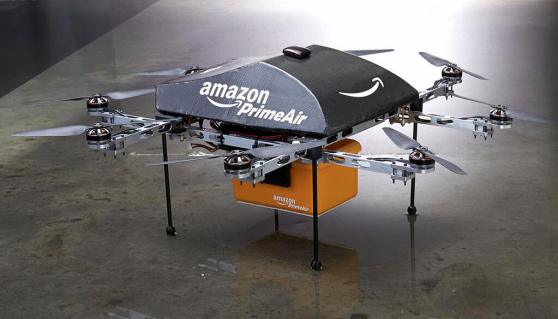
\includegraphics[width=0.4\textwidth]{amazon.jpg}\hspace{0.1\textwidth}
 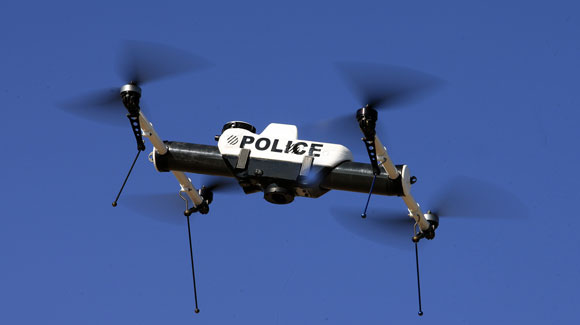
\includegraphics[width=0.4\textwidth]{police-drone.jpg}\\[2em]
 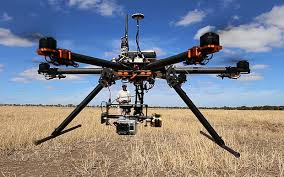
\includegraphics[width=0.4\textwidth]{gopro.jpg}\hspace{0.1\textwidth}
 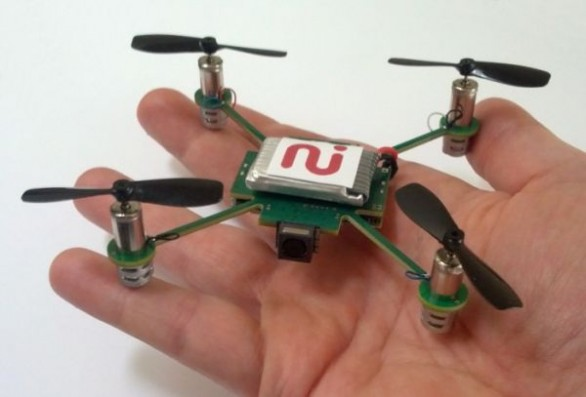
\includegraphics[width=0.4\textwidth]{microcopter.jpg}\par
 \caption{Different applications of multirotors}
 \label{figure:applications}
\end{figure}


As stated before, the uses of this platform are many and limited
only by the imagination of the designers. Figure \ref{figure:applications} illustrates various application going from search and rescue to public defense, most of them in outdoor scenarios. Very interesting is to investigate the possible use of this technology in an indoor scene where the comforting signal of the GPS is not present and analyze every aspect of flight going from state estimation, control and stability to autonomy, path planning and high level automation. \\*

This work investigates the integration between different heterogeneous entities as well as the possibility to design a safe, reliable and flexible architecture capable of letting the robot navigate safely in an indoor environment. At the end a simple algorithm for landing on a mobile platform is presented with very interesting results demonstrating the potential of this setup.

\subsection{Hosting laboratories}
This thesis is carried out as a cooperation between the Laboratorium Lab (focus:
autonomous robotics and ambient intelligence), the NOCC Lab (focus: control,
identification and estimation) and the EMARO@DIBRIS Lab.

\newpage

\section{Problem statement}

The goal of this master thesis to develop algorithms for UAV trajectory planning and execution (as well as the related SW components), using the motion capture system as the source of the UAV position feedback. Once achieved stability more complex aspects are investigated, a task based software architecture is presented and a simple technique for landing on a mobile platform is proposed.
The above stated, is formulated in to the following problem statement for the project: \\*

\noindent
\textbf{It is possible, through position feedback given from a motion capture system, to design a set of algorithms and SW components enabling the IRIS to achieve stability and perform different tasks in an indoor scenario? }

\subsection{Work plan}
The work got through several tasks covering all aspects, they can be distinctly divided in main blocks hence defining the work plan.

\begin{enumerate}

\item Analysis of state of the art approaches to UAV control, modeling, trajectory planning and execution

\item Technical analysis and documentation on the given tools (Autopilot, Motion Capture, IRIS Quadcopter)

\item Integration between mocap and IRIS
\begin{itemize}

\item Integration and testing between mocap and onboard estimation modules
\item Integration and testing of onboard controller through set point control

\end{itemize}

\item Design of the high level software architecture 
\item Testing the software, coding and debugging different kind of tasks
\item Design and testing an algorithm for landing on a mobile platform

\end{enumerate}
















